\section{Ejercicio 3}

\subsection{Problema}

El enunciado nos pide, dadas N esquinas y M calles bidireccionales resolver Q queries de varios tipos:
\begin{itemize}
	\item[A: ] dadas dos esquinas e1 y e2, imprimir la cantidad de calles que en caso de ser cortadas impiden llegar de e1 a e2.
	\item[B: ] dada una calle, imprimir un 1 si al cortar la calle existen al menos dos esquinas entre las que deja de haber un camino, y 0 en caso contrario.
	\item[C: ] dada una esquina e1, imprimir la cantidad de esquinas e2 tales que de cortar una sola calle, sea cual sea, seguir\'a habiendo camino de e1 a e2.
\end{itemize}

El modelo que se plantea entonces es representar las esquinas y calles como nodos y aristas respectivamente, de un grafo no dirigido
(porque las calles son bidireccionales).\\

Se asegura que el grafo es conexo (pues hay un camino para cada par de esquinas) y que hay una cantidad positiva de nodos y aristas.
Además, no hay calles que conectan las mismas esquinas, por lo cual no habrá ejes repetidos. \\

Debido a la complejidad que nos piden y que el grafo es conexo (hay al menos tantos aristas como vértices menos uno) y el algoritmo y nociones
vistas en clase para calcular Componentes Biconexas Maximales vamos a querer representar los aristas del grafo como listas de adyacencia para asi 
recorrer los nodos del grafo en tiempo lineal con respecto a la cantidad de aristas mediante DFS. Luego mas adelante se ve que las queries se resuelven
calculando puentes y otras propiedades entre los nodos del grafo mediante DFS. \\

Finalmente se debe imprimir el resultado de cada query segun su tipo, lo cual explicamos en detalle en la sección de Correctitud. \\

\subsection{Algoritmo e intuición}

\subsubsection*{Pseudocódigo}

Sea la clase $Grafo = <Vertices, Aristas, ListaAdyacencia>$
	donde Vertices y Aristas son Enteros que representan la cantidad de vertices y aristas del grafo y
	ListaAdyacencia es un $Vector<Lista<Par<Entero, Entero>>>$ donde
	el tamano del vector es Vertices y por cada arista que conecta nodos v 
	y w del grafo representado, ListaAdyacencia[v] incluye $<e, w>$ y
	ListaAdyacencia[w] incluye $<e, v>$ donde $e$ es el número de arista (entre 0 y Aristas-1).

\begin{algorithm}[]
    \caption{ResolverQueries}
    \Input{Grafo $grafo$, Queries $queries$}
    $Vector<Bool>$ $puentes \gets [false,...,false]$ con size grafo.Aristas \;
	$Vector<Entero>$ $depth \gets [-1,...,-1]$ con size grafo.Vertices \;
	$Vector<Entero>$ $low \gets [-1,...,-1]$ con size grafo.Vertices \;
	\emph{CalcularPuentesDFS$(grafo, puentes, depth, low, 0, 0, 0)$} \;
	$Vector<Entero>$ $componente\_puente\_del\_vertice \gets [-1,...,-1]$ con size grafo.Vertices \;
	$Vector<Entero>$ $vertices\_del\_componente\_puente \gets [0,...,0]$ con size grafo.Vertices \;
	$Variable$ $Global$ $Entero$ $contador\_componentes \gets 0$ \;
	\emph{CalcularComponentesPuenteDFS$(grafo, puentes, componente\_puente\_del\_vertice, $ $ vertices\_del\_componente\_puente, 0, contador\_componentes, 0)$} \;
	\For{$query$ en $queries$} {
		\If{$query.tipo$ == A} {
			$Vector<Bool>$ $visitado \gets [false,...,false]$ con size grafo.Vertices \;
			\emph{Imprimir PuentesEntreNodos$(grafo, puentes, visitado, query.esquina1, query.esquina2, query.esquina1)$}
		}
		\If{$query.tipo$ == B} {
			\emph{Imprimir $puentes[query.calle]$}
		}
		\If{$query.tipo$ == C} {
			$Entero$ $n$ \;
			$n \gets vertices\_del\_componente\_puente[componente\_puente\_del\_vertice[query.esquina]]$ \;
			\emph{Imprimir n-1}
		}
	}
\end{algorithm}

\begin{algorithm}[]
    \caption{CalcularPuentesDFS}
    \Input{Grafo $grafo$, Vector$<Bool>$ $puentes$, Vector$<Entero>$ $depth$, Vector$<Entero>$ $low$, Entero $v$, Entero $d$, Entero $padre$}
    $depth[v] \gets d$ \;
	$low[v] \gets d$ \;
	\For {$<e, w>$ en $grafo.ListaAdyacencia[v]$ tal que $w$ != $padre$} {
		\eIf{$depth[w]$ == -1}{
			\emph{CalcularPuentesDFS$(grafo, puentes, depth, low, w, d+1, v)$} \;
			$low[v] \gets min(low[v], low[w])$ \;
			\If {$low[w] >= depth[w]$} {
				$puentes[e] \gets true$
			}
		}{
			$low[v] \gets min(low[v], depth[w])$ \;
		}
	}
\end{algorithm}

\begin{algorithm}[]
    \caption{CalcularComponentesPuenteDFS}
    \Input{Grafo $grafo$, Vector$<Bool>$ $puentes$, Vector$<Entero> componente\_puente\_del\_vertice$, Vector$<Entero> vertices\_del\_componente\_puente$, Entero $v$, Variable Global Entero $contador\_componentes$, Entero $componente\_actual$}
    $componente\_puente\_del\_vertice[v] \gets componente\_actual$ \;
    $vertices\_del\_componente\_puente[componente\_actual]++$ \;
    \For {$<e, w>$ en $grafo.ListaAdyacencia[v]$} {
    	\If {$componente\_puente\_del\_vertice[w]$ == -1} {
			\eIf {$puentes[e]$} {
				$contador\_componentes++$ \;
				$Entero$ $componente \gets contador\_componentes$ \;
				\emph{CalcularComponentesPuenteDFS($grafo, puentes, componente\_puente\_del\_vertice,$ 
				$vertices\_del\_componente\_puente, w, contador\_componentes, componente$)} \;
			}{
				\emph{CalcularComponentesPuenteDFS($grafo, puentes, componente\_puente\_del\_vertice,$ 
				$vertices\_del\_componente\_puente, w, contador\_componentes, componente\_actual$)}
			}
		}
    }
\end{algorithm}

\begin{algorithm}[H]
    \caption{PuentesEntreNodos}
    \Input{Grafo $grafo$, Vector$<Bool>$ $puentes$, Vector$<Bool>$ $visitado$, Entero $src$, Entero $dst$, Entero $actual$}
    $visitado[actual] \gets true$ \;
    \If {$actual == dst$} {
    	\Return{0}
    }
    $Entero$ $ans \gets -1$ \;
    \For {$<e, w>$ en $grafo.ListaAdyacencia[v]$} {
    	\If {$visitado[w]$ == $false$} {
			$Entero$ $rec \gets$ PuentesEntreNodos$(grafo, puentes, visitado, src, dst, w)$ \;
			\If{$rec$ != -1} {
				$ans \gets puentes[e]$ ? $rec+1$ : $rec$
			}
		}
    }
    \Return{ans}
\end{algorithm}

\subsubsection*{Estrategia}

Primero calculamos los ejes puentes con un algoritmo similar al que calcula Componentes Biconexas Maximales. Por esto
guardamos los ejes del grafo como lista de adyancecia y para cada eje guardamos su numero de eje (asi despues los podemos
marcar rapido como eje puente). Se recorre el grafo mediante DFS y asi podemos garantizar que su complejidad sera lineal 
con respecto a la cantidad de vertices y aristas. \\
Luego separamos los nodos en Bridge Components (explicación en la seccion siguiente). Esto lo hacemos tambien mediante DFS. \\
Finalmente contestamos cada query segun los datos calculados previamente excepto en el caso de las queries tipo A en cuyo caso 
se calculan los aristas puentes entre los nodos que representan las esquinas. Nuevamente usamos DFS. \\
A lo largo de todos los algoritmos vamos manteniendo vectores de longitud grafo.Aristas o grafo.Vertices para ir guardando resultados
parciales y nodos visitados en cada recorrido DFS del grafo. \\

\subsection{Correctitud}

\subsubsection*{ResolverQueries}
Esta es la función principal del algoritmo. Dado el grafo y las queries de entrada se crea un vector $puentes$ 
que contiene para cada arista si es puente o no, lo cual se quiere calcular a continuaci\'on. \\
Es importante notar que por la forma en que se crea la clase Grafo y se rellena, cada eje tiene un número 
único entre 0 y la cantidad de aristas menos uno. \\
Luego se crean dos vectores $depth$ y $low$ de tamaño cantidad de vértices del grafo. Con esto se calculan los
ejes puente mediante la funci\'on CalcularPuentesDFS. El nodo inicial de CalcularPuentesDFS es arbitrario 
mientras sea el mismo que el padre inicial, por lo cual se define al nodo 0 como el inicial. Además queremos 
que el $depth$ inicial sea 0 ya que es la profundidad inicial de los nodos según el algoritmo para calcular 
Componentes Biconexas Maximales explicado en clase, que es en definitiva el esquema que sigue la funcio\'n 
CalcularPuentesDFS. \\
Habiendo calculado los aristas puente, ahora se quiere calcular para cada nodo e1, la cantidad de nodos e2 
tales que de cortar una sola arista, sea cual sea, seguir\'a habiendo un camino de e1 a e2. \\
Como el grafo es conexo, las nodos inicialmente están conectados. Dada el nodo e1, si existe una arista tal que al 
cortarla e1 y otro nodo se desconectan entonces seguro que esa arista es un puente (por la definición de puente). 
De hecho, si corto una arista que no es puente, el grafo sigue siendo conexo. \\
El problema es cuando e1 y e2 forman un puente o pertenecen a diferentes componentes biconexas maximales, es decir, 
cuando hay un puente entre ellos. Debido a eso, e1 y e2 siguen estando conectados no importa cual arista sea cortada
si y solo si pertenecen a una misma componente biconexa maximal que no sea un puente. \\
Entonces es posible seguir llegando de un nodo e1 a otro e2 habiendo cortado una calle 
cualquiera, mientras no hayan aristas puente entre ellos. Si hay un arista puente entre ellos, cortarlo basta para desconectarlos. \\
Con esta motivación definimos los Bridge Components del grafo. Estos componentes se obtienen condensando cada componente biconexa 
maximal que no es un puente en un solo nodo. \\

Ejemplo:\\
\begin{figure}[H]
\centering
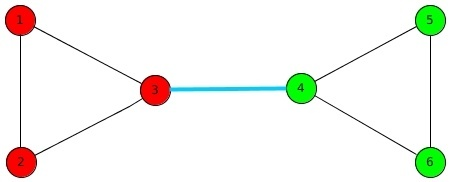
\includegraphics[width=90mm]{./img/bridge_comp_1.jpeg}
\caption{Grafo original}
\end{figure}
\begin{figure}[H]
\centering
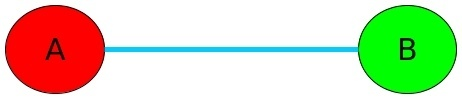
\includegraphics[width=90mm]{./img/bridge_comp_2.jpeg}
\caption{Grafo condensado en Bridge Components}
\end{figure}

El algoritmo CalcularComponentesPuenteDFS hace esto guardando para cada nodo 
a qué Bridge Component pertenece en el vector $componente\_puente\_del\_vertice$ y para cada uno de esos componentes, 
$vertices\_del\_componente\_puente$ guarda cuántos nodos tiene ese componente. \\
Ahora bien, los nodos dentro de cada Bridge Component están conectados de manera tal que no hay puentes entre ellos,
por lo cual si corto cualquier arista del grafo siguen estando conectados entre si.

Finalmente, el algoritmo resuelve las queries según su tipo correspondiente:
\begin{itemize}
	\item[A: ] dado que se quiere imprimir la cantidad de calles que, en caso de ser cortadas impiden llegar de la 
	esquina e1 a e2, cuenta mediante la función PuentesEntreNodos y el vector $puentes$, los puentes entre los nodos 
	del grafo que representan esas esquinas.
	\item[B: ] se fija en el vector $puentes$ si la calle es un puente o no y lo imprime.
	\item[C: ] dada una esquina e1 se quiere imprimir la cantidad de esquinas e2 tales que de cortar una calle cualquiera 
	sigue habiendo camino de e1 a e2. Como explicamos esto es exactamente la cantidad de nodos en el Bridge Component del
	grafo, que son justamente los nodos e2 que están conectados a e1 sin puentes entre e1 y e2, entonces sin importar
	qué calle se corte, seguirán estando conectados. Los demás nodos son posibles de desconectar de e1 cortando alguno
	de los aristas puentes entre e1 y esos nodos. Notar que a esta cantidad se le resta 1 para no contar a e1 en su 
	propio Bridge Component.
\end{itemize}

\subsubsection*{CalcularPuentesDFS}

Este algoritmo es casi idéntico al visto en clase para calcular Componentes Biconexas maximales. \\

Dados los vectores $puentes$, $depth$, $low$ va guardando mediante un recorrido DFS en:
\begin{itemize}
	\item $puentes$: para cada numero de arista, si ese arista es un puente.
	\item $depth$: la distancia del nodo actual al nodo raiz del arbol DFS mediante Tree edges.
	\item $low$: la menor distancia/$depth$ de la raiz del arbol DFS a la que el nodo actual puede saltar
	desde su sub-arbol de DFS con raiz en si mismo. \\
	Esto quiere decir que dado el nodo v: $low[v]$ = $\min(d[v], \min\limits_{y \in hijosDFS(v)} low[y], \min\limits_{backedge(v,w)} d[w])$
\end{itemize}

Para calcular los $low$ se va recorriendo mediante DFS la lista de adyacencia de los nodos y para cada nodo:
\begin{itemize}
	\item Si es no visitado (nos fijamos que $depth$ de ese nodo no sea -1) hacemos una llamada recursiva con el nodo
	actual ahora como padre y al Entero $d$ le sumamos 1 indicando que en el arbol de DFS actual ese nodo
	estará a un nodo de distancia más de la raiz del arbol. Después actualizamos el $low$ del nodo actual
	como el mínimo entre este y el del nodo hijo que visitamos ya que si un hijo puede llegar a un nodo
	mas cercano a la raiz del arbol, el nodo actual también. \\
	$Observaci\acute{o}n (clase)$: Un tree-edge del nodo v a uno de sus hijos w es puente si y solo si, low[w] $\ge$ depth[w], es decir, 
	no existe ning\'un back-edge que permita salir del sub\'arbol con ra\'iz en w.
	\item Si el nodo fue visitado (es ancestro en el arbol de DFS) actualizamos el $low$ del nodo actual
	como el mínimo entre este y el $depth$ nodo ancestro ya que es un back-edge.
\end{itemize}

El algoritmo en si solo difiere con el visto en clase en que en vez de ir guardando puentes, puntos de 
articulación y reportar componentes biconexas maximales, solo guardamos los aristas puentes. \\

$Observaci\acute{o}n$: el grafo tiene que ser conexo para devolver todos los puentes (pero sabemos por la entrada que lo es). \\

$Observaci\acute{o}n$: el parámetro $d$ inicial siempre es 0 porque es la distancia de la raiz a si misma. \\

$Observaci\acute{o}n$: si bien el nodo inicial (que será la raiz del arbol DFS) es arbitrario, se quiere que
este sea el nodo 0 ya que el problema nos asegura solamente que hay al menos un nodo en todo el grafo. \\

\subsubsection*{CalcularComponentesPuenteDFS}

Como explicamos anteriormente, en este algoritmo vamos a querer calcular por cada nodo a qué Bridge Component pertenece
y cuantos nodos tiene cada Bridge Component. \\

Habiendo ya calculado los aristas $puentes$ esto se resuelve de la siguiente manera:
\begin{itemize}
	\item Mantenemos en el vector $componente\_puente\_del\_vertice$ el Bridge Component al que pertenece cada nodo.
	\item Mantenemos en el vector $vertices\_del\_componente\_puente$ cuántos nodos tiene cada una de estas componentes
	(notar que son a lo sumo grafo.Vertices componentes porque los Bridge Components particionan los nodos del grafo).
	\item Tenemos un valor $componente\_actual$ que va a ir cambiando a medida de que en el recorrido DFS pasamos por un arista puente.
	\item Tenemos una variable global $contador\_componentes$ que, cuando pasamos por una arista puente en el DFS (es decir, cambiamos
	de componente) usamos para tomar un nuevo n\'umero de componente para asignarle asi nunca tenemos repetidos.
	\item En el recorrido DFS, para cada nodo $v$ recorremos su lista de adyancecia y por cada nodo $w$ no visitado
	($componente\_puente\_del\_vertice[w]$ == -1) si el arista que los conecta es un puente hacemos un llamado recursivo cambiando el
	Bridge Component y en caso contrario hacemos un llamado recursivo con el mismo Bridge Component.
\end{itemize}

Recorrer el grafo de esta manera usando DFS efectivamente agrupa los nodos en Bridge Components porque de antemano se sabe cuales son 
los aristas $puentes$ y entonces el DFS llega hasta cada nodo que no pasa por un puente con el mismo valor de $componente\_actual$ (si
cambia de componente es porque habia un puente y ya no se puede volver mediante DFS a un componente anterior sin pasar por ese puente). \\

$Observaci\acute{o}n$: el grafo tiene que ser conexo para recorrer todos los Bridge Components (pero sabemos por la entrada que lo es). \\

\subsubsection*{PuentesEntreNodos}

Devuelve para un par de nodos $src$ y $dst$ la cantidad de puentes entre ellos. \\

Esto se hace recorriendo mediante DFS el grafo con las listas de adyancecia de cada nodo y manteniendo los visitados en el vector
$visitado$. \\
Es importante tener en cuenta que en el arbol DFS del grafo hay un unico camino simple entre cada par de nodos (porque es un arbol)
y que este camino entonces va a pasar por todos los  aristas puentes entre $src$ y $dst$ (porque el arbol DFS necesariamente contiene
a todos los aristas puentes del grafo, sino se desconecta). \\
De esta manera se recorre cada nodo (mantenido en el parámetro $actual$ del algoritmo, que inicialmente debe ser $src$)
hasta llegar al destino $dst$. Por cada arista voy sumando 1 a la cantidad de puentes si el arista es un puente y cuando llego a $dst$ 
(es decir cuando el nodo $actual$ es el $dst$) devuelvo 0. Si no se puede llegar al nodo destino mediante nodos no visitados devuelvo -1
para indicar que se fallo. \\

$Observaci\acute{o}n$: los nodos $src$ y $dst$ tienen que estar conectados para que el algoritmo funcione pero esto ya lo sabemos
porque el grafo es conexo de entrada. \\

\subsection{Complejidad}

Sea N la cantidad de esquinas/nodos del grafo y M la cantidad de calles/aristas del grafo nos piden un algoritmo con complejidad
$O(M+MQ_A+Q_B+Q_C)$ donde $Q_X$ es la cantidad de queries de tipo $X$. \\

Como el grafo es conexo sabemos que $O(N) \subseteq O(M)$ (porque M es al menos N-1). \\

CalcularPuentesDFS hace un recorrido DFS del grafo para calcular los ejes puentes de la misma forma que el algoritmo para calcular
Componentes Biconexas Maximales que vimos en clase es $O(N+M)$ porque cada nodo se recorre una sola vez a través de llamados recursivos
y, aparte de esto, solo se realizan asignaciones y comparaciones. Como se vio antes $O(N) \subseteq O(M)$, entonces $O(N+M) \subseteq O(M)$.  \\

CalcularComponentesPuenteDFS hace un recorrido DFS como en CalcularPuentesDFS y podemos saber los nodos ya visitados mediante el vector
$componente\_puente\_del\_vertice$ por lo cual recorremos cada nodo una sola vez y cada arista lo consideramos solo en los ciclos For de
los nodos que conecta. Aparte de los llamados recursivos que componen el DFS solo hay asignaciones y comparaciones, por lo cual la funci\'on
es $O(N+M) \subseteq O(M)$. \\

PuentesEntreNodos también hace un recorrido DFS como las dos funciones anteriores y mantiene los nodos visitados en el vector $visitado$. Aparte
de esto solo se realizan comparaciones y asignaciones, por lo que esta funci\'on tambi\'en tiene complejidad $O(N+M) \subseteq O(M)$. \\

ResolverQueries (el algoritmo principal):
\begin{itemize}
	\item Crea 5 vectores de longitud $O(N)$ o bien $O(M)$, ambos siendo $O(M)$. Entonces la complejidad de crearlos es $O(5M) \subseteq O(M)$.
	\item Hace un llamado a la funci\'on CalcularPuentesDFS que tiene complejidad $O(M)$.
	\item Hace un llamado a la funci\'on CalcularComponentesPuenteDFS que tiene complejidad $O(M)$.
	\item Por cada query de tipo A creamos un vector de longitud $O(N) \subseteq O(M)$ y se hace un llamado a 
	PuentesEntreNodos que es $O(M)$. En total por cada query de tipo A se hace trabajo $O(M+M) \subseteq O(M)$. Como
	hay $Q_A$ queries de tipo A, estas conllevan una complejidad de $O(MQ_A)$.
	\item Por cada query de tipo B solo se tiene que imprimir un valor ya calculado de un vector, lo cual es $O(1)$. Como
	hay $Q_B$ queries de tipo B, estas conllevan una complejidad de $O(Q_B)$.
	\item Por cada query de tipo C solo se realizan comparaciones y asignaciones, lo cual es $O(1)$. Como
	hay $Q_C$ queries de tipo C, estas conllevan una complejidad de $O(Q_C)$.
\end{itemize}

Por lo tanto, teniendo en cuenta los 6 items previos, la complejidad final es $O(M+M+M+MQ_A+Q_B+Q_C) \subseteq O(M+MQ_A+Q_B+Q_C)$, tal y como
se pide en el enunciado.

\subsection{Casos de prueba}
